\section{Local Data Management}

This section explains how FLOps handles local data on learner nodes.
Firstly, it covers what kind of data and datasets suit FL and why.
Secondly, it discusses how state-of-the-art projects in the industry handle enormous amounts of data for ML and Big Data applications.
Thirdly, it explores how exactly FLOps manages the local data and what architecture it uses for this task.
The last subsection showcases FLOps' mock data provider service, which makes development and testing more convenient.

\subsection{Appropriate Data for FL}

FL, especially cross-device FL, specializes in massive numbers of heterogeneous devices with diverse non-IID data.
For FL, one can use conventional datasets, such as MNIST or CIFAR10.
However, such homogeneous and IID data is not representative of data found on real devices.
Many works in the field of FL specialize and compare how well they perform on non-IID data (\ref{subsection:fl_research}).
For this reason, various datasets and benchmarks have been created explicitly for FL.
One recurring prominent FL benchmarking tool is LEAF \cite{paper:leaf_fl_benchmark}.
It does not solely specialize in FL but in more general federated settings.
It includes several implementations and datasets.
As mentioned in Table \ref{table:fl_research_table_2}, we had little success working with this benchmark.
This finding is noteworthy because LEAF seems to be the primary and sole source for the FEMNIST dataset, which many FL papers mention and use for evaluation.

FEMNIST seems to be one of the most popular dedicated FL benchmarking datasets.
It is a federated version of the Extended MNIST (EMNIST \cite{emnist_dataset}) dataset.
FEMNIST splits the EMNIST dataset into multiple classes or data partitions based on individual (digit/symbol) writers.
Extended projects exist that wrap the access to FEMNIST via the high-speed HDF5 binary data format \cite{hdf5_femnist}.
The FEMNIST dataset is a prominent example of many dedicated FL datasets and benchmarks.
A detailed listing and comparison of other similar resources is available in \cite{thesis:tum_fl_framework_comparison}.

FLOps requires a convenient way of accessing suitable data for development and testing purposes.
Our experience trying out LEAF taught us that using these dedicated datasets can be challenging and error-prone.
Instead of figuring out how to unify these different dedicated FL datasets and benchmarks, we use Flower Datasets \cite{flower:datasets}.
We already discussed Flower Datasets briefly in \ref{subsection:flower}.
The vital thing to know about this young project is that it uses and splits up Hugging Face datasets into non-IID data fragments.
It enables users to turn conventional ML datasets into FL-optimized ones.
Users can configure this approach freely.

\subsection{ML \& Big Data Formats}

The field of Big Data and ML formats is vast and complex.
It provides many insights into different optimization approaches.
Great resources to find out more are available here \cite{influxdb_apache_stack,apache_arrow_flight_sql_2022,columnar_roadmap_parquet_and_arrow,apache_arrow_flight_intro}.
The following are significant takeaways after investigating this domain.
\vspace{5mm}
\newline
\textbf{Managing Big Data is a booming Field}\newline
Storing and handling Big Data is a massively popular, expensive, and profitable business that regularly attracts hundred-million-dollar investments.
This environment leads to healthy competition, solid standards, and bold advancements in the field.
\vspace{5mm}
\newline
\textbf{Reuse}\newline
Data management and optimizations are universally needed.
These areas have several decades of solid research to back up best practices and avoid known pitfalls.
Similarly to security, one should avoid reinventing and reimplementing foundational features from the ground up.
Instead, it is recommended that existing open-source industry-favored solutions be reused.
\vspace{5mm}
\newline
\textbf{(De)Serialization is a critical Bottleneck}\newline
When each subsystem has its own internal memory format, significant amounts of CPU work get wasted on (de)serialization.
The recommended way to avoid this is to stick to a uniform format.
The more tools support such a uniform format, the easier and faster cooperation, communication, and transmission can be.
\vspace{5mm}
\newline
\textbf{Big Data and ML Data should use Columnar Formats}\newline
Usually, dataset features are split up into different columns.
These features can be diverse and require different data types for storage.
When storing and handling conventionally stored row-wise data, all these different data types and features complicate and slow down processing.
Instead, if the data is stored and handled column-wise, advanced optimizations, and compressions can handle homogeneous features and their data type.
As a result, the same data can be processed more compactly and faster.
\vspace{5mm}
\newline
The sources above recommend the following open source state-of-the-art formats and technologies.
All of them are from Apache.
\vspace{5mm}
\newline
\textbf{Arrow}\newline
Arrow is a language-agnostic columnar memory format.
It is optimized for modern CPUs and GPUs.
It supports zero-copy reads, which avoid serialization and accelerate data access.
Arrow is especially popular for interoperability.
This format should be used for data in memory. \cite{arrow_repo} 
\vspace{5mm}
\newline
\textbf{Parquet}\newline
Parquet is also a columnar file format.
Its focus is on efficient data storage and retrieval.
Its benefit over Arrow is that it needs less space due to its special compression and encoding.
This format should be used to store data on disks. \cite{docs:parquet}
\vspace{5mm}
\newline
\textbf{Arrow Flight}\newline
Arrow Flight is a gRPC-based framework.
It supports parallel data streams.
When used with compatible data, it overcomes (de)serialization overheads and speeds up data transfer.
Flight should be used to transport Apache formatted data over the network. \cite{docs:arrow_flight}
\vspace{5mm}
\newline
The last subsection mentioned that FLOps uses Flower Datasets, which uses Hugging Face Datasets underneath.
Hugging Face Datasets use Arrow \cite{docs:hugging_face_arrow}.
Therefore, the findings in this subsection are directly applicable and relevant to FLOps.

\subsection{FLOps' Local Data Management Architecture}
\begin{figure}[h]
    \begin{adjustwidth}{-0.1\paperwidth}{-0.1\paperwidth}
        \centering
        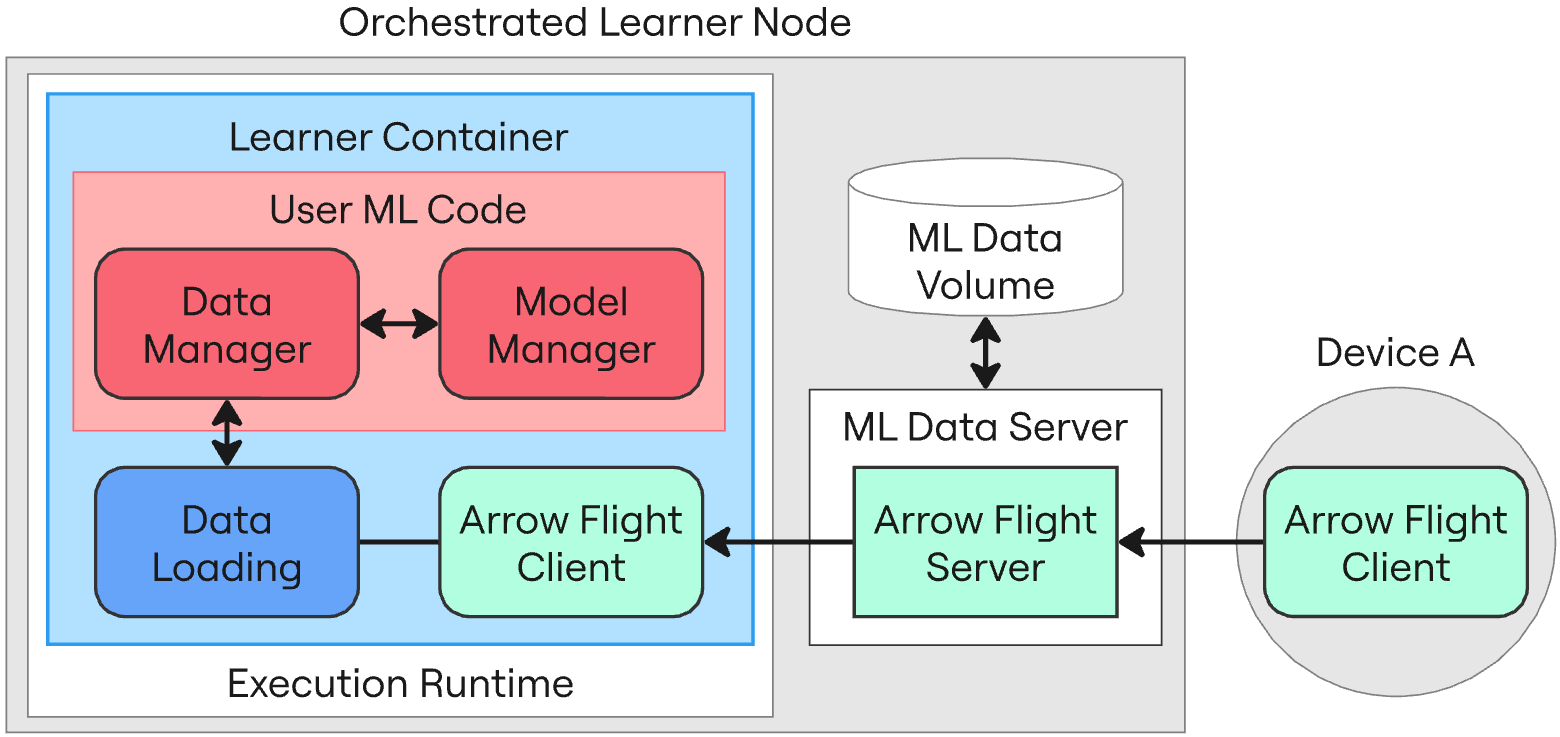
\includegraphics[width=0.80\paperwidth]{local_data_loading_medium.png}
        \caption{FLOps Local Data Management Structure}
        \label{fig:medium_local_data_management}
    \end{adjustwidth}
\end{figure}
Figure \ref{fig:medium_local_data_management} depicts the architecture of FLOps' local data management.
The important concretions compared to the simplified version in Figure \ref{fig:flops_simple_data_management} from \ref{subsection:flops_overview} are as follows:
The learner container and the data-providing device must have an Arrow Flight client installed and connected to the Arrow Flight server in the ML data server.
The data loading component in the learner uses the Flight client to retrieve the matching data.
It gets added by the builder service and is not part of the user's ML code.
The data and model manager utilize this loaded data.
Note that the figures in this subsection depict a single data source device for optimizing page space.
Arbitrary many devices are supported by this setup.

\begin{figure}[p]
    \begin{adjustwidth}{-0.1\paperwidth}{-0.1\paperwidth}
        \centering
        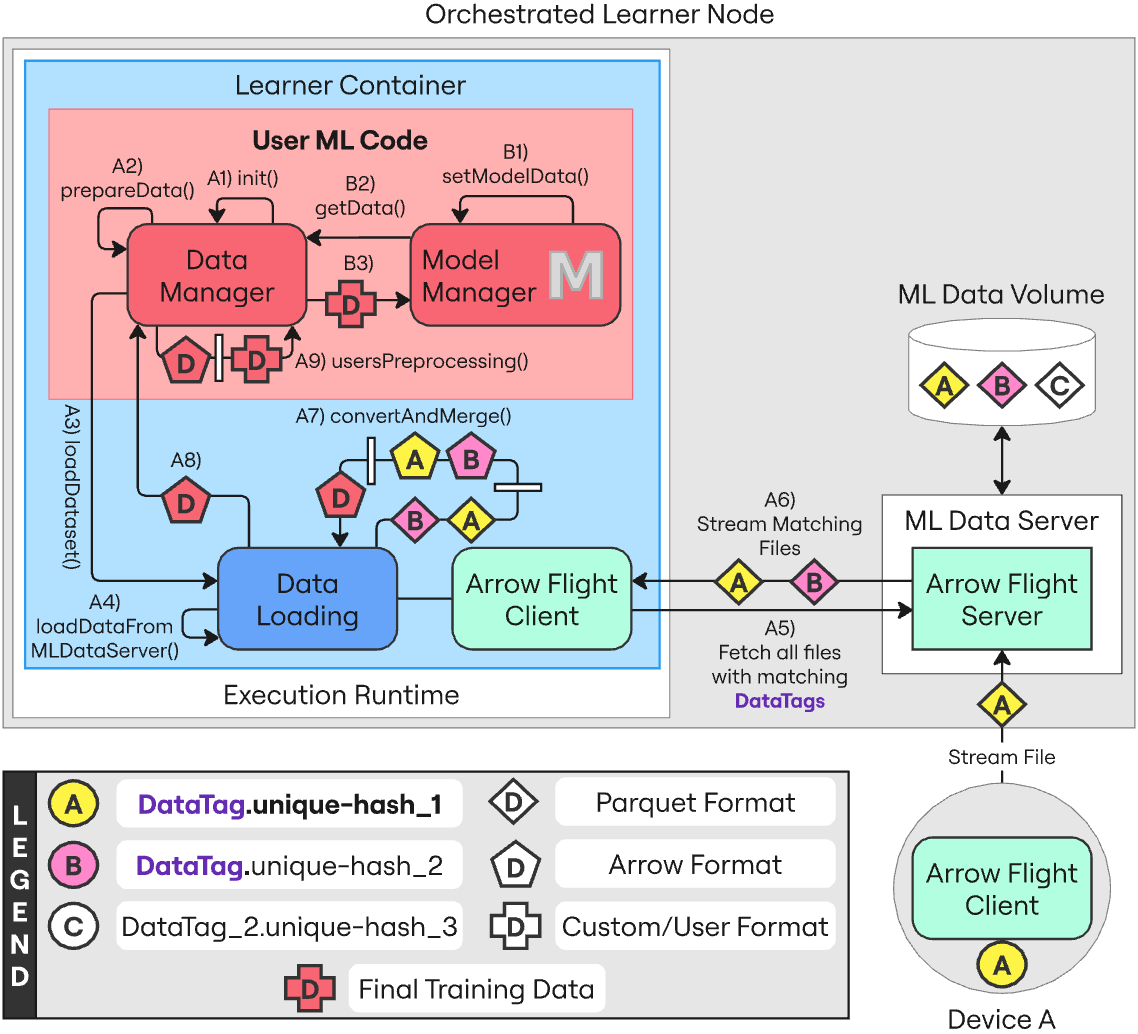
\includegraphics[width=0.90\paperwidth]{local_data_loading_detailed.png}
        \caption{Detailed FLOps Local Data Management Structure}
        \label{fig:detailed_local_data_management}
    \end{adjustwidth}
\end{figure}
Figure \ref{fig:detailed_local_data_management} depicts FLOps' local data management processes in more detail.
Firstly, the unique data resides on device A.
The device can store its data in an arbitrary format.
The device trusts the learner node in its proximity and transfers its data A to its ML data server via Flight.
For this, it needs to convert its data into Parquet format.
Secondly, the ML data server receives this streamed data and stores it locally on the learner node in a dedicated ML data volume.
This volume now contains several different Parquet files from different sources.
It uses Parquet files based on the last subsection's recommendations.

The next sequence of steps starts from the user's data manager.
During its initialization (A1), when the learner service is run, it triggers its \texttt{prepareData} function (A2).
This method calls the wrapper/adapter function \texttt{loadDataset} (A3).
The \texttt{loadDataset} function calls the \texttt{loadDataFromMLDataServer} function (A4).
This function is not available for users during development.
It is instead injected by the builder service, so it is exclusively available in the learner image's augmented FL code.

The Data Loading's \texttt{loadDataFromMLDataServer} function contacts its Flight client to request all matching files from the local ML data server (A5).
The match is performed based on the user's project SLA.
This SLA includes a \texttt{dataTags} key that is a list of string tags.
When devices send over their files, they must provide a data tag.
The ML data server will store these data files in the format seen in the Figure's legend.
The name starts with a singular data tag and ends with a unique hash based on the file's content.
Users and data providers need to cooperate to ensure that these data tags match.
The ML data server takes all files which name's prefix matches the user requested SLA data tags and streams them over into the learner container (A6).
In the example shown, only data files A and B have matching data tags.
The Flight server streams both over to the data-loading component.

Now that the matching data files are available inside the learner container, they must be transformed to fit the user's needs.
The data loading component converts its received Parquet files into Arrow format (A7) for better in-memory data management.
Usually, ML code expects and works with whole datasets instead of multiple split ones.
For this reason, the data loading component also merges its received files into a single dataset (A7).
The data loading component then sends this dataset to the user's data manager (A8).
The data manager now has access to the necessary dataset and can perform custom preprocessing and transformation steps (A9).
Users can freely configure and implement this preprocessing to ensure the retrieved data is usable for their ML model.

When FL training starts, the user's model manager will initially set the model data (B1).
Its \texttt{getData} method (B2) contacts the data manager and returns its prepared compatible dataset (B3).
In conclusion, these steps enable FLOps to manage and provide real local FL data to diverse user ML code for training and evaluation.

\subsection{Mock Data Providers}

Coordinating and managing real data providers while developing or testing can be challenging.
FLOps offers its own mock data providers to make these processes more convenient.
These optional services can be deployed on learner nodes via the orchestrator.
They split datasets into partitions and send them to the ML data server exactly as real devices.
It is enough to run them once to populate the local learner nodes with data.
These mock data providers also act as implementation examples for real devices when converting data, setting up a Flight client, and communicating with an ML data server.
The code is available here \cite{flops_code}.
Subsection \ref{subsection:api} shows the API endpoint for creating such mock data providers.
The FLOps Helper SLA for mock data providers looks as follows:
\begin{lstlisting}
    {   % The ID has to match the user's orchestrator ID.
        "customerID": "Admin",
        "mock_data_configuration": {
            % This value can be any dataset name available in Hugging Face.
            "dataset_name": "cifar10",
            "number_of_partitions": 1,
            "data_tag": "cifar10" 
        }
    }
\end{lstlisting}
\begin{figure}[h]
    \begin{adjustwidth}{-0.1\paperwidth}{-0.1\paperwidth}
        \centering
        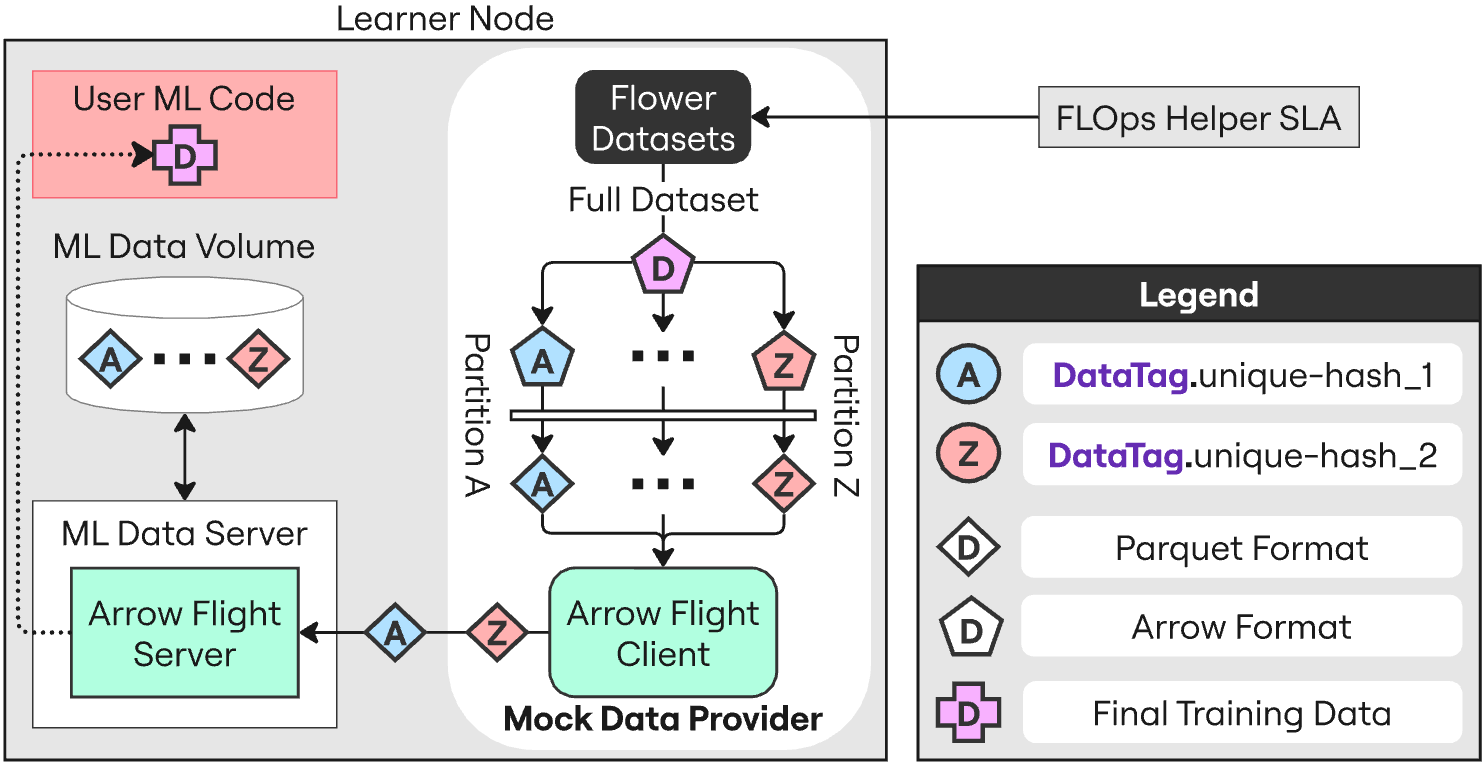
\includegraphics[width=0.80\paperwidth]{mock_data_provider.png}
        \caption{FLOps' Mock Data Provider}
        \label{fig:mock_data_provider}
    \end{adjustwidth}
\end{figure}
Figure \ref{fig:mock_data_provider} depicts FLOp's mock data provider.
The mock data provider runs as an orchestrated service in the container execution environment, similar to the learner service.
It uses the requested Hugging Face dataset name to download the dataset via Flower Datasets.
The data provider uses Flower Datasets to split this monolith dataset into multiple partitions.
The user defines the number of partitions.
Each partition is individually sent to the ML data server as if real edge devices were contacting the server.
The ML data server stores each partition separately in the ML data volume.
Ultimately, these partitions will be merged and preprocessed to be fit for training.

